%**************************************************************
% ocsvm
%**************************************************************
\subsection{One-Class Support Vector Machine}
    In questa sottosezione, esaminiamo il modello basato sull'apprendimento automatico One-Class Support Vector 
    Machine\cite{ocsvm} (OC-SVM) come altro punto di riferimento per valutare le prestazioni del modello 
    MSCRED\cite{mscred}. La scelta del modello OC-SVM è motivata dalla sua ampia utilizzazione nella 
    letteratura di riferimento e dal suo impiego da parte dei ricercatori di MSCRED per il confronto delle 
    prestazioni. In generale, gli algoritmi di tipologia Support Vector Machine sono noti per offrire buone 
    prestazioni in diversi contesti. Tuttavia, tendono a soffrire quando si tratta di classificazione di 
    anomalie, poiché le anomalie costituiscono solitamente una piccola parte del dataset, creando uno 
    sbilanciamento tra le classi.

    \paragraph{Intuizione} OC-SVM, come gli altri algoritmi della famiglia SVM, opera tracciando confini 
    decisionali tra i dati. Nell'ambito della rilevazione delle anomalie, questo si traduce nella definizione 
    di un iperpiano che separa i punti considerati anomali da quelli considerati non anomali.

    \paragraph{Dataset} Nell'esperimento è stato suddiviso il dataset di riferimento negli insiemi di training, 
    validation e test con le stesse percentuali utilizzate per ARMA, ovvero $0.5, 0.182, 0.318$ rispettivamente. 
    La \hyperref[tab:dataset-ocsvm]{Tabella 3.2.} mostra la percentuale di anomalie in ciascun 
    sottoinsieme del dataset originale, mentre nella \hyperref[fig:dataset-div1]{Figura 3.4.} viene
    evidenziato il dataset partizionato.


    \begin{table}[H]
        \centering
        \caption{Statistiche dataset OC-SVM.}
        \begin{tabular}{lccc}
            \toprule
            \textbf{Dataset} & \textbf{Indice di suddivisione} & \textbf{\# punti} & \textbf{Anomalie (\%)} \\
            \toprule
            \textbf{Training}   & 0.5   &  24168 & 2.01\% \\
            \textbf{Validation} & 0.182 &  8797  & 8.60\% \\
            \textbf{Testing}    & 0.318 &  15372 & 9.59\% \\
            \bottomrule
        \end{tabular}
        \label{tab:dataset-ocsvm}
    \end{table}

    \begin{figure}[H]
        \centering
        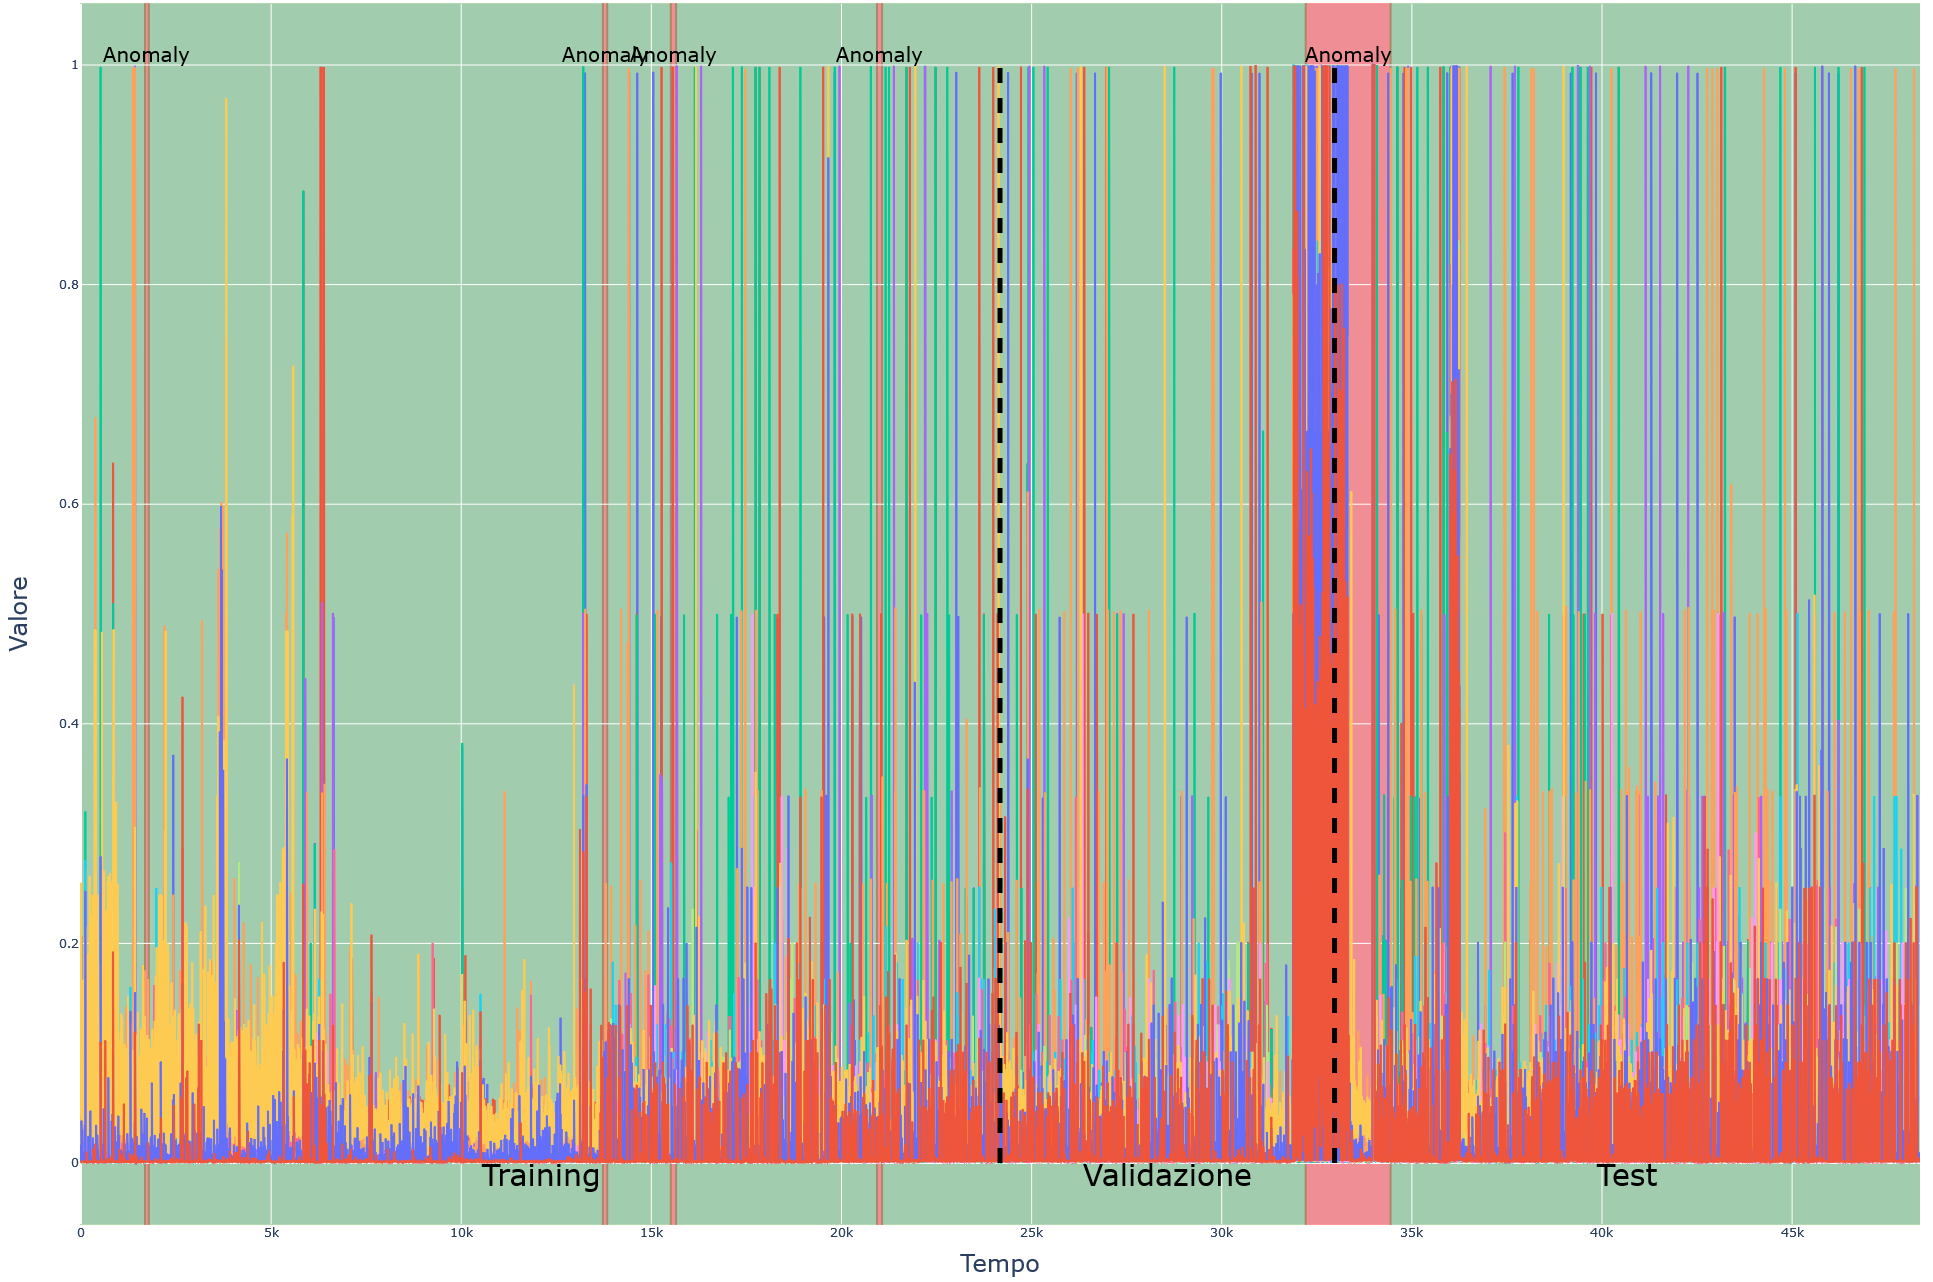
\includegraphics[width=0.5\textwidth]{./input/chapters/models/figs/dataset_div1.png}
        \caption{Suddivisione dataset negli insiemi di training, validation e test. Le due linee 
        tratteggiate rappresentano, da sinistra a destra rispettivamente la suddivisione tra l'insieme di training e 
        validazione e tra l'insieme di validazione e test.}
        \label{fig:dataset-div1}
    \end{figure}


    \begin{table}[H]
        \centering
        \caption{Valori candidati per gli iperparametri.}
        \begin{tabular}{lccc}
            \toprule
            \textbf{Iperparametro} & \textbf{Candidati} \\
            \toprule
            $\nu$ & 0.03, 0.1, 0.25, 0.5, 0.9 \\
            \midrule
            Kernel & linear, poly, rbf, sigmoid \\
            \bottomrule
        \end{tabular}
        \label{tab:iperparametri-candidati}
    \end{table}

        \paragraph{Iperparametri} Gli iperparametri $\nu$ e il tipo di kernel sono stati trovati effettuando una 
        "grid-search" partendo 
        da un insieme di candidati per entrambi gli iperparametri illustrati nella 
        \hyperref[tab:iperparametri-candidati]{Tabella 3.3.} La combinazione di valori $(\nu^*, \text{Kernel}^*)$ che 
        ha massimizzato lo score F1 sul validation set è stata scelta come configurazione ottimale.

        Formalmente, siano $\mathbf{Tr}, \mathbf{Va}$ i dataset utilizzati per il training e
        per il validation rispettivamente e sia $\text{OC-SVM}_\mathbf{X}^\mathbf{Y}$ un modello OC-SVM addestrato
        su $\mathbf{X}$ che effettua previsioni sulle etichette dei punti $\mathbf{Y}$ e sia $K$ l'insieme dei 
        possibili valori che può assumere il kernel, ossia $K=\{\text{linear}, \text{poly}, \text{rbf}, \text{sigmoid}\}$:


    \begin{equation}
        \label{eq:ocsvm-problem}
        \begin{aligned}
            & \nu^*, \text{Kernel}^* = \max_{\nu, \text{Kernel}} F1(\text{OC-SVM}_\mathbf{Tr}^\mathbf{Va}(\nu, \text{Kernel})) \\
            & \text{con il vincolo} \quad \nu \in [0.03, 0.1, 0.25, 0.5, 0.9], \text{Kernel} \in K
        \end{aligned}
    \end{equation}
        
        \paragraph{Soluzione} \hyperref[eq:ocsvm-problem]{L'equazione 3.2}  è stata soddisfatta dai seguenti valori:
        \begin{itemize}
            \item $\nu^* = 0.9$
            \item Kernel$^* = \text{sigmoid}$
        \end{itemize}

        Dopo aver utilizzato l'insieme di validazione esclusivamente per l'ottimizzazione degli iperparametri, 
        è stato poi unito al dataset di addestramento. Successivamente, il modello è stato addestrato sul nuovo
        dataset combinato, utilizzando gli iperparametri che hanno prodotto una soluzione ottimale durante la fase di 
        convalida. In \hyperref[fig:ocsvm-sol]{Figura 3.5.} viene mostrata la 
        soluzione dopo l'applicazione di PCA per fornire una rappresentazione ai primi tre componenti principali.
        
        \begin{figure}[H]
            \centering
            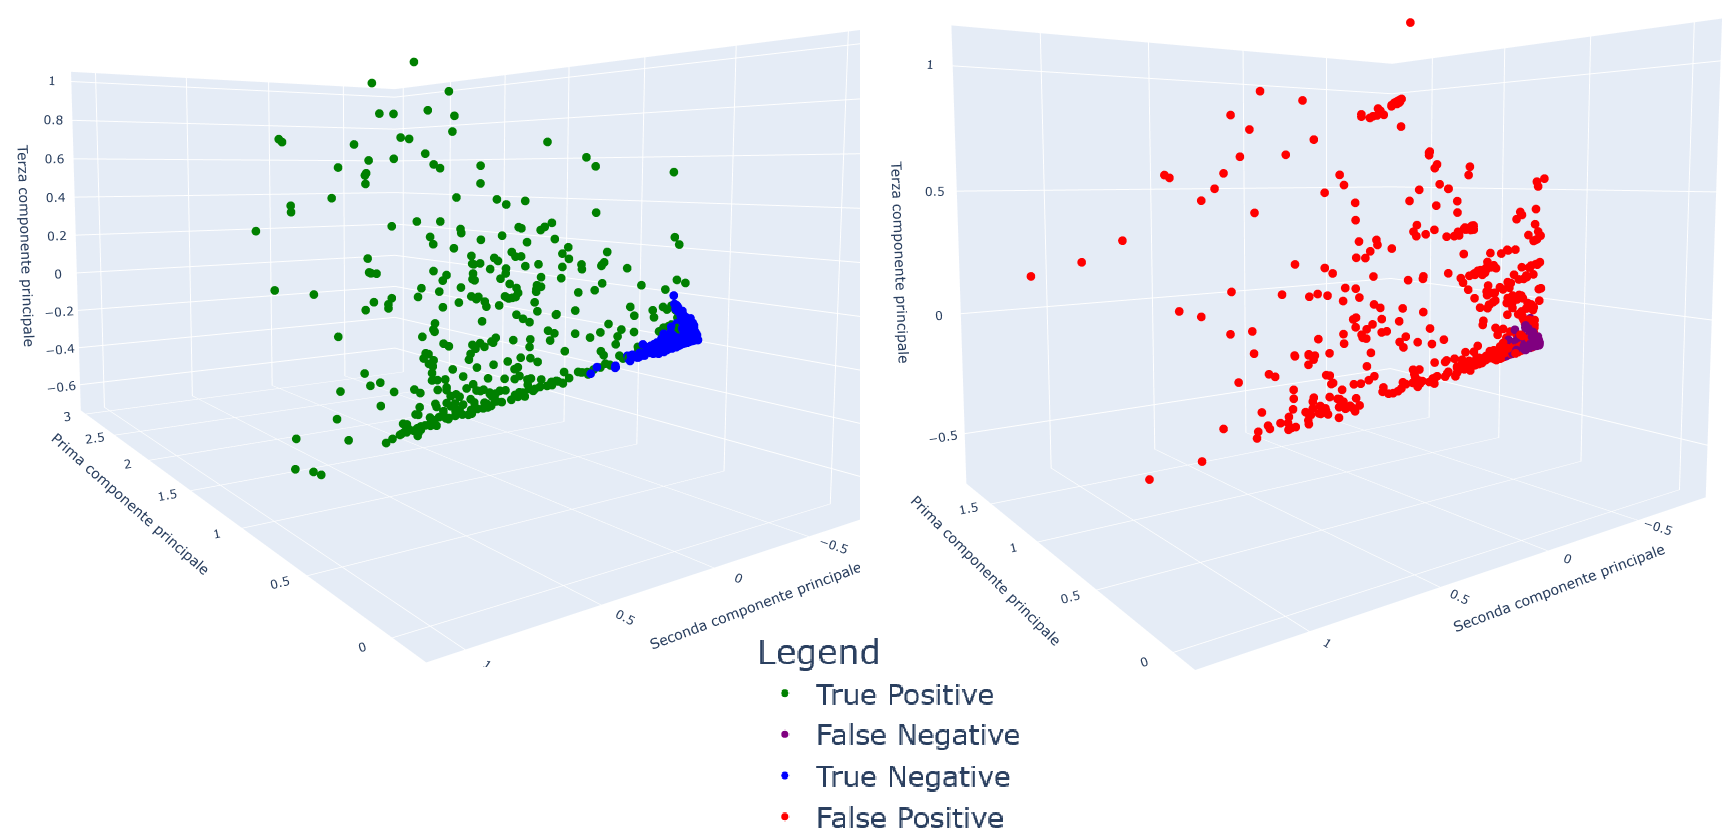
\includegraphics[width=0.7\textwidth]{./input/chapters/models/figs/ocsvm-sol.png}
            \caption{\small
                Soluzione del modello OC-SVM dopo l'applicazione di PCA ai primi tre 
                componenti principali, garantendo una rappresentazione visibile rispetto a quella 
                originale a dodici dimensioni. A sinistra sono rappresentate le previsioni corrette
                (TP, TN), mentre a destra quelle errate (FP, FN).
            }
            \label{fig:ocsvm-sol}
        \end{figure}

        I risultati mostrano chiaramente che il modello ha prestazioni scarse sul dataset di test. 
        I punti verdi a sinistra della \hyperref[fig:ocsvm-sol]{Figura 3.5.} sono quelli classificati correttamente 
        come anomalie (True Positives) e quelli blu sono quelli classificati correttamente come non anomali (True Negatives). 
        Tuttavia, molti punti sono stati classificati in modo errato, come evidenziato a destra nella stessa figura. 
        I punti viola rappresentano le anomalie erroneamente classificate come normali (False Negatives), 
        mentre i punti rossi sono i punti normali erroneamente classificati come anomalie (False Positives).  
        
